% ===================================================================
% Solution results, rewritten 2026-06-26 to the honest non-identifiability
% framing (docs/CLAIMS_v2.md). The retracted thesis ("the observational
% estimator recovers a reliable poison-negative the write-back gate needs")
% is GONE. Numbers: 4B-campaign macros from numbers_solution.tex
% (experiments/analyze_campaign.py over results/campaign_v2/); the
% gold-standard LOO + positive control + ladder numbers are lab-scale and
% inlined with per-number provenance comments (same convention as the
% theorem section). Every inline number traces to a committed artifact.
% ===================================================================

We instantiate the credit signals on the recalibrated corpus
(\S\ref{sec:setup}): \textbf{B0} (no memory), \textbf{B2} (static similarity
retrieval), \textbf{outcome} (the bandit with outcome credit), and
\textbf{observational} (the online observational causal bandit, \S\ref{sec:onl}); an
active leave-one-out re-rollout (\S\ref{sec:active}) serves as the assumption-light
\emph{gold standard} against which we judge the cheap signals. Each learning condition
streams the \CampNtrain{} training challenges for \CampEpochs{} epochs, is then frozen,
and is evaluated paired against the others on the \CampNheldout{} held-out instances
over \CampEvalSeeds{} seeds. The held-out set and seeds are identical across
conditions, so every contrast below is within-item paired (bootstrap CI + exact
McNemar). Rows are instance$\times$seed and seeds are positively correlated, so these
campaign $p$-values are anti-conservative; no campaign-level contrast is claimed
significant. The gold-standard re-rollout, the positive control, and the capability
ladder are established at \emph{lab scale} on the same instrument (the high-$n$
campaigns, e.g.\ \texttt{campaign\_14b\_M3\_powered}, $n{\approx}15.6$k); we say so at
each use. One provenance caveat: the 4B campaign itself ran on an earlier benchmark
revision (poison-contract / oracle-labeling / grid-duplication bugs fixed later in commit
\texttt{63db02d}) and was \emph{not} re-run, so the 4B magnitudes below are illustrative of
the failure mode---the load-bearing non-identifiability evidence is the lab-scale ladder,
not the 4B numbers.

\paragraph{The boundary, reproduced on real logs.} Outcome credit cannot tell an
executed-but-recovered-from poison lesson from a useful one. Over the full training
stream it learns a mean $Q$ of \OutQTrue{} for true lessons and \OutQPoison{} for
poison: it ranks true lessons only slightly higher (gap
\OutQGap{}, $n{=}4$/label---too few for a formal test) and assigns poison
a clearly \emph{positive} value, because a verifiable success credits whichever lesson
was in context and the poison's claimed action (\texttt{base64}) is part of the correct
recipe it cannot be denied credit for. An outcome-credit memory therefore holds no
internal signal that executed poison is anything but a useful lesson---the failure mode
this paper is about.

\paragraph{The free experiment identifies the \emph{helpful} lessons.} The same logs
contain a free randomized experiment: each lesson's inclusion is a stochastic draw with
a logged propensity (\S\ref{sec:obs}). Re-scoring \emph{those same} outcome-condition
runs with the observational SNIPW estimator (\S\ref{sec:obs})---no extra inference---recovers
the value of the helpful lessons outcome credit conflates with poison: the mean IPW ATE
on reward is \ObsAteTrue{} for true lessons, a large positive effect, with distractors
at \ObsAteDistract{}. This large helpful effect is where the agent's own exploration
\emph{does} suffice to credit a lesson causally for free, and it is corroborated by the
gold standard: at lab scale the active re-rollout ranks the helpful lessons in strong
agreement with the cheap estimate (within-helpful rank correlation $+0.64$, CI
$[+0.34,+0.85]$; the gold
standard orders $30/30$ helpful nodes)%
\footnote{Lab-scale, \texttt{campaign\_14b\_M3\_powered}; emitted by
\texttt{experiments/within\_poison\_validation.py} into \texttt{active\_loo\_within\_label.json}.}
and the helpful on-target solve ATE (the \emph{on-target} contrast restricts the run
set to challenges of the lesson's own family---family is pre-treatment---as opposed to the
\emph{marginal-inclusion} effect of merely placing it in the retrieved $M$-set) is large at every rung and markedly larger at the
high-capability Qwen rungs
($+0.247/{+}0.195/{+}0.526/{+}0.570/{+}0.227$ at 3B/7B/14B/32B/Llama-8B, all $p<.001$;
\S\ref{sec:identifiability}). This is the \emph{positive} half of the boundary.

\paragraph{\ldots but not the per-item harm of a poison lesson.} The negative half is
the paper's central result. The same observational estimator reads poison only
\emph{mildly} negative---\ObsAtePoison{} on this 4B campaign, and at higher capability
with far more data a small $-0.057$ ($p{<}.001$, CI $[-0.087,-0.022]$) at 14B and $-0.064$
($p{=}.005$, CI $[-0.109,-0.018]$) at 32B---the pre-registered per-rung primary contrast
at each rung; the 14B/32B cells survive Benjamini--Hochberg at $q{=}.05$ across the five
rungs, the other rungs are null (all other grid cells are exploratory). These are the \emph{on-target} contrasts; the marginal-inclusion ATE is null at
every $M$ (\S\ref{sec:disc}).%
\footnote{Lab-scale on-target SNIPW, \texttt{campaign\_14b\_M3\_powered} and \texttt{campaign\_32b\_M3\_tp2}
(\S\ref{sec:identifiability}).}
That sign is \emph{not} the per-item causal harm (Fig.~\ref{fig:sep}). Against the assumption-light active
leave-one-out gold standard---which re-solves each challenge with and without a single
lesson, holding the others fixed---the cheap estimate cannot \emph{rank} the per-item
poison effect: within poison, the rank correlation between the cheap estimate and the
gold standard is $\approx 0$ ($+0.072$ tie-corrected Spearman, $+0.028$ rank-Pearson;
wide bootstrap CI $[-0.35,+0.49]$, emitter-backed, seed 0), and among the lessons the
gold standard can order
at all, the two agree on the \emph{sign} of only $8$ of $18$ ($p{=}0.76$, one-sided
exact binomial against chance $0.5$---at chance,
not anti-correlated).%
\footnote{\texttt{experiments/within\_poison\_validation.py}; the often-quoted ``$8/28$''
counts $10$ gold-standard ties-at-zero (a $1/12$-quantized estimate) as disagreements.}
The reason is not merely that the cheap estimator is noisy: the feasible-$n$ gold
standard \emph{itself} cannot resolve the small poison effects. Its mean poison marginal
is $+0.045$ ($n{=}28$ lessons), $95\%$ CI $[-0.006,+0.098]$---a fail-to-reject,
\emph{ill-posed}, never a
measured ``zero''---and its per-node standard error (a worst-case $p{=}0.5$ binomial
bound at the deployed re-roll budget, $\approx0.20$) exceeds the between-node spread of
the effects it must rank ($0.14$). \textbf{Neither} signal
identifies the per-item harm---and if anything this understates the difficulty: the
active-LOO contexts themselves rendered the poison lesson \emph{first}, biasing its
per-item effect toward looking \emph{more} harmful, so the gold standard's inability to
rank it is conservative. The mildly-negative observational sign is a real
\emph{label-level} regularity but a confounded one---\S\ref{sec:identifiability} derives
its source under the measured base-rate floor---and it is neither the per-item causal
estimand nor, as we show below, a signal a write-back gate can be built on.

\paragraph{A positive control: what verifiable credit \emph{can} catch.} The
non-identifiability is specific to a \emph{benign}-false lesson the agent recovers from,
not a blanket failure of the estimator. We additionally plant two \emph{actively
destructive} lesson types that push the outcome \emph{below} the base-rate
floor---one that destroys working state (\textsf{destroy}) and one that burns the round
budget (\textsf{exhaust})---a \textsf{wrongflag} lesson that confidently submits a wrong
answer, and a deterministic \textsf{verifier} that re-runs the cited recipe in
isolation. The SNIPW estimator \emph{detects} the floor-violating harms
(\textsf{destroy} ATE $\MalPoolDestroyAte{}$, two-sided $p{=}\MalPoolDestroyPtwo{}$,
CI $\MalPoolDestroyCI{}$, $\MalPoolDestroyNfam{}$ families; \textsf{exhaust}
$\MalPoolExhaustAte{}$, $p{=}\MalPoolExhaustPtwo{}$, CI $\MalPoolExhaustCI{}$,
$\MalPoolExhaustNfam{}$ families; both CIs excluding $0$, though the binary
\textsf{destroy} clears $p<.05$ only once campaigns are pooled---see note) but is \emph{untested} on \textsf{wrongflag}. The
agent executed that recipe on only $11$ of $453$ sampled runs (follow rate $0.024$,
against $0.978$ and $0.805$ for \textsf{destroy} and \textsf{exhaust}), so its
on-target SNIPW ($+0.004$, $p{=}.69$, $64$ families---the same pooled estimator and file
as \textsf{destroy}/\textsf{exhaust} above,
\texttt{malignant\_pooled\_combined.json}) carries almost no treated exposure: this
is a null from non-exposure, not a demonstrated blind spot. Under \emph{forced} exposure
the constructed leave-one-out does detect the arm ($-0.43$, CI $[-0.54,-0.32]$, $n{=}41$
families; direction and sign only---see note).\footnote{The \textsf{wrongflag} arm was
already toothless at the pre-registered probe---cited on $0$ of $42$ sampled runs
(\texttt{campaign\_14b\_malig\_probe/merged/malignant\_probe\_check.json})---which the
pre-registration required be redesigned before scaling. It was scaled unmodified; we log
this as a deviation and treat the arm as untested rather than as evidence of a blind
spot.} The execution-verifier flags invalid recipes on $100\%$ and valid ones on $0\%$ of
families \emph{by construction} (a deployable contrast on \emph{recipe validity}, not a
measured generalization; \S\ref{sec:identifiability}, Prop.~\ref{thm:recovery}). The
malignant campaign over-samples its planted lessons ${\sim}2.5\times$, which depresses the
base rate and makes the \emph{same-campaign} benign poison read spuriously positive
(run-level $+0.033$, one-sided $p{=}.0475$, two-sided $.095$)---so the benign-poison null is the
\emph{main}-campaign result, not this one---but \textsf{destroy}/\textsf{exhaust} are
floor-\emph{violating} and detected regardless.%
\footnote{Lab-scale malignant campaign, family-clustered SNIPW \emph{pooled} over
\texttt{campaign\_14b\_malig} + \texttt{campaign\_14b\_malig\_expand} ($74$/$71$ family
clusters in the \textsf{destroy}/\textsf{exhaust} contrasts);
the single-campaign binary \textsf{destroy} was borderline ($p{=}.057$) and the campaign
was expanded to power it, so the robust single-campaign evidence is the descriptive
within-family \textsf{destroy} ATE $-0.045$, CI $[-0.055,-0.032]$ (excludes $0$ without
pooling). The constructed direct-harm magnitudes are forced-exposure and
order-confounded, so they are direction/sign evidence, not clean effect sizes.}
This is the boundary in one experiment: outcome-based credit identifies large helpful
effects and actively-destructive harm, but \emph{not} the per-item harm of a
benign-false lesson, and it is \emph{untested} against a confidently-wrong answer.

\begin{figure}[t]
\centering
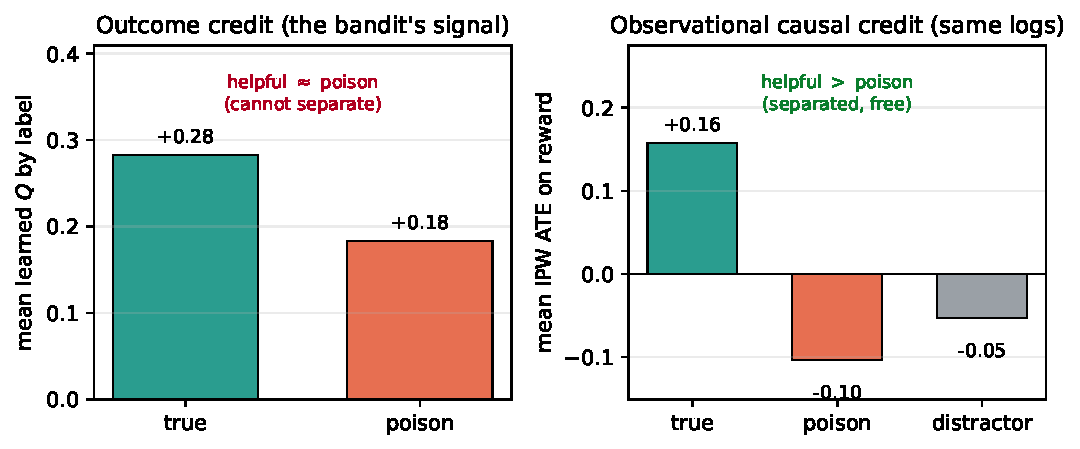
\includegraphics[width=0.92\linewidth]{fig_separation.pdf}
\caption{Same logs, two credit signals (4B recalibrated campaign, run on the earlier
pre-fix benchmark revision; magnitudes illustrative).
\emph{Left:} outcome-bandit $Q$ by ground-truth label---executed poison earns a positive
value, numerically beside true lessons. \emph{Right:} observational IPW ATE on the same
runs---poison mildly negative, true strongly positive. The mild negative is a confounded
label-level sign, \emph{not} a per-item poison detector (\S\ref{sec:identifiability}).}
\label{fig:sep}
\end{figure}

\paragraph{Held-out solve rate (parity, by design).} Table~\ref{tab:solve} reports
solve rates; the headline is \emph{not} here, and the next paragraph explains why it
should not be. Retrieval is directionally ahead of no memory (B2 \CampBtwo{} vs.\ B0
\CampBzero{}, paired \BtwoVsBzero{}, $p\eqd\BtwoVsBzeroP{}$---underpowered here; the
pilot's paired lift, \S\ref{sec:results}, is the significant version of this contrast),
consistent with the
recalibrated corpus putting the solver in a band where lessons matter. But the credit signals are not separated at this $n$: the
online observational causal bandit reaches \CampObs{} against the outcome bandit's
\CampOutcome{} (paired \ObsVsOutcome{}, McNemar $p\eqd\ObsVsOutcomeP{}$) and static
retrieval's \CampBtwo{} (paired \ObsVsBtwo{}). Whatever the credit signal, the bandit
retrieves the true lesson and the solver follows it, so solve rate does not separate
the signals---and, as we have shown, neither does any of them recover the per-item
poison effect.

\begin{table}[t]
\centering\small
\setlength{\tabcolsep}{5pt}
\begin{tabular}{lc}
\toprule
condition & held-out solve \\
\midrule
B0 (no memory)       & \CampBzero{} \\
B2 (static)          & \CampBtwo{} \\
outcome credit       & \CampOutcome{} \\
observational causal & \CampObs{} \\
\midrule
paired contrast & $\Delta$ (McNemar $p$) \\
\midrule
B2 $-$ B0                  & \BtwoVsBzero{} ($p\eqd\BtwoVsBzeroP{}$) \\
observational $-$ outcome  & \ObsVsOutcome{} ($p\eqd\ObsVsOutcomeP{}$) \\
observational $-$ B2       & \ObsVsBtwo{} ($p\eqd\ObsVsBtwoP{}$) \\
\bottomrule
\end{tabular}
\caption{Top: held-out solve rate by credit signal (4B campaign, run on the pre-fix
benchmark revision and not re-run---illustrative; see the provenance caveat opening
\S\ref{sec:results2}). Bottom: within-item paired
contrasts (McNemar). Retrieval lifts solve over no memory, but the credit signals
are not separated on solve rate at this $n$ (an underpowered fail-to-reject, not a measured
equality; both paired intervals are bounded above by $0.0$) (and, as the text shows, in any trustworthy
per-item poison value).}
\label{tab:solve}
\end{table}

\paragraph{Where the harm does and does not surface.} The credit signals are at parity
on \emph{immediate} held-out solve rate, expected on the \emph{marginal} retrieval
distribution: a capable solver follows the true lesson whenever it is co-retrieved and
ignores a co-retrieved false one, so a false lesson does not lower immediate solve in
single-step retrieval. Two qualifications keep this honest. First, under \emph{forced}
co-presence in a tight round budget, adding a poison lesson alongside the true one
\emph{does} lower solve, by ${\approx}0.31$---but this effect is \emph{not} a per-item
constant (poison alone is mildly recoverable-\emph{positive}, $+0.05$, CI excluding $0$,
floor-bounded at base ${\approx}0.04$;
difference-in-differences $-0.37$) and it is resource/co-presence-mediated: against a
pure budget-burner (\textsf{exhaust}) control, poison hurts \emph{no more}---poison$-$%
\textsf{exhaust} is $+0.042$ ($p{=}.78$) on the solvable subset (a cannot-reject-equality,
underpowered at $n{=}15$---\emph{not} a formal equivalence (TOST) test) and $+0.204$
($[+0.040,+0.357]$, $p{=}.0164$) over all $41$ families (poison hurts \emph{less}
than the maximal burner). Disclosed:
those constructed rollouts rendered the poison lesson \emph{first} (a primacy confound,
since fixed), so we do not headline the magnitude.%
\footnote{\texttt{experiments/crypto\_interference\_analysis.py} over
\texttt{constructed\_loo\_crypto.json}; the order-neutral renderer
(\texttt{solver/context\_assembly.py}, content-hash order) is the fix.}
The reading consistent with the gold standard is that there is no clean, order-robust
\emph{per-item} poison value---further support for the non-identifiability result, not a
separate harm. Second, the small negative is an \emph{on-target} (family-restricted)
contrast, \emph{not} the marginal-inclusion ATE: conditioned on a poison lesson actually
being executed, the solve rate dips a measurable $-0.0745$ ($p<.001$) at full exposure
($M{=}1$) within crypto, while the causal marginal-inclusion ATE stays null at every
breadth ($M{=}1$ $-0.021$, $p{=}.25$). We treat this conditional sub-floor harm as the
strongest rival reading, which we name in
\S\ref{sec:disc}.

\paragraph{Does the confounded sign make a usable gate? No.} It is tempting to read the
observational poison-negative as a write-back filter. Applied as a promote-if-positive
gate to each signal's learned values on the \emph{same} outcome-condition logs, it would
admit \PromotePoisonOut{} of the planted poison under outcome credit and
\PromotePoisonObs{} under the observational value. We report this only to \emph{disavow}
it as a deployable result: the gate ``works'' here solely because the observational sign
happens to be negative on these four lessons, and that sign is exactly the confounded,
non-identifiable quantity the gold standard cannot reproduce (within-poison rank
correlation $\approx0$); the $0\%$ figure is itself fragile---the same observational
estimator admits $25\%$ of the poison when read off the \emph{observational}-condition logs
rather than these outcome-condition ones---and the lab-scale causal gate is only
\emph{partially} label-selective, at a real cost: at 14B it promotes
$\PromoHelpCausalFourteenB{}$ of the helpful nodes but only
$\PromoPoisonCausalFourteenB{}$ of the poison (Fisher $p{=}6.8{\times}10^{-4}$), and
$\PromoHelpCausalThirtyTwoB{}$ against $\PromoPoisonCausalThirtyTwoB{}$ at 32B
($p{=}.004$), while at 7B it does not separate the labels at all
($\PromoHelpCausalSevenB{}$ vs.\ $\PromoPoisonCausalSevenB{}$, $p{=}1.0$; likewise null
at 3B, $\PromoHelpCausalThreeB{}$ vs.\ $\PromoPoisonCausalThreeB{}$, and Llama-8B,
$\PromoHelpCausalLlamaB{}$ vs.\ $\PromoPoisonCausalLlamaB{}$). For comparison the
outcome gate promotes essentially everything ($\PromoHelpOutFourteenB{}$ helpful and
$\PromoPoisonOutFourteenB{}$ poison at 14B). That separation is the same confounded
\emph{label-level} regularity, not the per-item ranking a gate needs---and buying it
costs between a quarter and a half of the helpful nodes at the two selective rungs, and
about half at the three where it does not separate. With four lessons and a
sign we have shown is \emph{not} the causal estimand, this is an illustration of the
failure mode, not a working suppressor. A trustworthy gate would need a signal that ranks
the per-item poison effect, which---in this regime---neither the cheap estimator nor the
gold standard provides. Whether \emph{any} oracle-free signal can gate benign-false lessons, and the
downstream cross-challenge solve-rate cost of propagated poison at scale, is the open
problem we name in \S\ref{sec:disc}.
